\section{Rozwój postaci gracza (Bartosz Strzelecki)}\label{s:impl_progres}
W implementacji systemu rozwoju postaci zastosowano system, w którym gracz zdobywa doświadczenie związane z daną statystyką
zgodnie z tabelą \ref{fig:prog}. Po osiągnięciu pewnego progu, który jest liniowo zależny od dotychczasowego poziomu danej umiejętności,
gracz uzyskuje korzyści ze zwiększonego poziomu statystyki. Po poprawieniu umiejętności postaci gracza na ekranie jest pokazywany odpowiedni
komunikat (rys. \ref{fig:modal}) informujący użytkownika o nowo nabytych zdolnościach.


\begin{figure}[htbp]
    \centering
    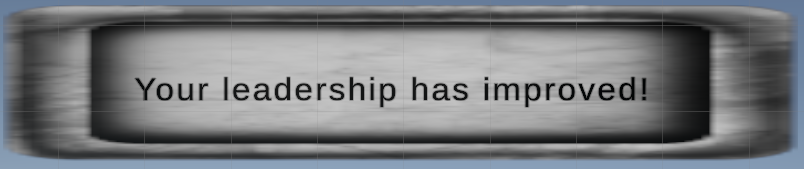
\includegraphics[width=0.8\textwidth]{images/modal}
    \caption{Komunikat informujący gracza o zdobyciu kolejnego poziomu umiejętności.}\label{fig:modal}
\end{figure}
